\documentclass[ansiapaper]{report}
\usepackage[utf8]{inputenc}
\usepackage[english]{babel}
\usepackage[T1]{fontenc}
\usepackage{amsmath}
\usepackage{amsfonts}
\usepackage{amssymb}
\usepackage{makeidx}
\usepackage{graphicx}
\usepackage{float}
\usepackage{lmodern}
\usepackage[dvipsnames]{xcolor}
\usepackage{tikz}
\usetikzlibrary{intersections}
\usepackage{pgfplots}
\usetikzlibrary{calc}
\usepackage[ansiapaper]{geometry}
\geometry{hmargin=2cm,vmargin=2cm}
\usepackage{fancybox}
\usepackage{mathtools}
\usepackage{enumitem}
\usepackage{tcolorbox}
\usepackage{colortbl}
\usepackage{fancybox}
\tcbuselibrary{most}
\usepackage{pifont}
\usepackage[skip = 5pt, font = {footnotesize}, labelfont = sl]{caption}
\usepackage{subcaption}
\usepackage{eso-pic}
\usepackage{nicematrix}
\usepackage{multicol}
\usepackage{booktabs}
\usepackage{svg}
\usepackage{derivative}
\usepackage{wrapfig}
\usepackage{stmaryrd}
\usepackage{yfonts}
\usepackage{array}
\usepackage{csquotes}
\usepackage[style=nature , backend=biber]{biblatex}
\addbibresource{bibliography.bib}
\author{Andrea}
\setlength{\columnsep}{.5cm}
\usepackage[explicit]{titlesec}
\usepackage{lipsum}
\usepackage{indentfirst}
\usepackage{tabularx}
\usepackage{amsmath}
\usepackage{fancyhdr}
\usepackage{etoolbox}
\usepackage[export]{adjustbox}
\usepackage{fourier-orns}
\usepackage{lettrine}
\usepackage{physics}
\usepackage{hyperref}
\usepackage[titletoc]{appendix}
\usepackage{adforn}
\usepackage{cmbright}
\usepackage{wrapfig}
\definecolor{MyRed}{RGB}{197,112,93}
\definecolor{MySand}{RGB}{208,184,168}
\definecolor{MyWhite}{RGB}{248, 237, 227}
 %% Option 'familydefault' only if the base font of the document is to be sans serif
% use Roman numerals for sections
% \renewcommand\familydefault{\rmdefault}
\renewcommand{\thesection}{\Roman{section}}

% use Arabic numerals for subsections
\renewcommand{\thesubsection}{\Alph{subsection}}

% use letters for subsubsections with a parenthesis
\renewcommand{\thesubsubsection}{\alph{subsubsection})}

% put a period and space after numbers
\titlelabel{\thetitle\thickspace}

% % Make section titles centered and bold
\titleformat{\section}[block]
  {\MakeUppercase\normalsize\sffamily\bfseries}
  {\thesection .}{.3em}
  {\color{black}#1}

  \titleformat{\subsection}[block]
  {\centering\small\sffamily\bfseries}
  {\thesubsection .}{.3em}
  {\color{black}#1}

  \titleformat{\subsubsection}[block]
  {\small\sffamily\bfseries}
  {\thesubsubsection }{.3em}
  {\color{black}#1}
% \titleformat*{\subsection}{\bfseries}

\titleformat{\paragraph}[hang]
{\small\sffamily\slshape}
{\theparagraph}{.3em}
{\color{MyRed}#1}


\titleclass{\chapter}{straight}
\titleformat{\chapter}[block]
{\color{white}\large\sffamily\bfseries}
{}
{0em}
{\colorbox{MyRed}{\parbox{\dimexpr\linewidth-2\fboxsep\relax}{\centering \space#1}}}
[]
\titlespacing{\chapter}{0pt}{5pt}{5pt}
\titlespacing{\section}{0pt}{*3}{*3}
\titlespacing{\subsection}{0pt}{*1.5}{*1.5}
\titlespacing{\subsubsection}{0pt}{*1.5}{*1.5}


\hypersetup{
    colorlinks=false,
    linkbordercolor = {white},
    menubordercolor = {white},
    citebordercolor = {black},
    urlbordercolor = {black},
}
\captionsetup{singlelinecheck=off, box=colorbox,boxcolor=MyRed!20, labelsep=endash}

\pgfmathdeclarefunction{gauss}{2}{%
  \pgfmathparse{1/(#2*sqrt(2*pi))*exp(-((x-#1)^2)/(2*#2^2))}%
}
\usetikzlibrary{decorations.markings}
% \renewcommand{\headrule}{%
% \vspace{6pt}\hrulefill
% \raisebox{0pt}{\quad\adforn{64} \adforn{8} \adforn{36}\quad}\hrulefill}
% Page style setup
\pagestyle{fancy}
\fancyhf{} % Clear all header and footer fields

% Set the header height
\setlength{\headheight}{1cm}

% Custom header setup
\fancyhead[L]{%
    \begin{tikzpicture}[overlay, remember picture]
        \node[anchor=north west, xscale=1, yscale=1, minimum width=.7\paperwidth, minimum height=\headheight, fill=MyRed, text=white, inner sep=0pt, outer sep=0pt, line width=0pt] at ([yshift=-0.7cm]current page.north west) {\parbox[c][\headheight]{.7\paperwidth}{\sffamily{\hskip2cm \textbf{\leftmark \hfill \small{Master SdM}\hspace{.5cm} }}}};
        \node[anchor=north east, xscale=1, yscale=1, minimum width=.2\paperwidth, minimum height=\headheight, fill=white, text=MyRed, inner sep=0.5pt, outer sep=0pt, line width=0pt] at ([yshift=-0.7cm, xshift=-1cm]current page.north east) {\parbox[c][\headheight]{.3\textwidth}{\centering\sffamily{\textbf{\small{ENS | ENSL}}}}};
        \draw[MyRed, line width=0.3mm]
        ([yshift=-0.7cm, xshift=-1.75cm]current page.north east)
        rectangle ([xshift=-\paperwidth*0.3+.5cm, yshift=-1.65\headheight-0.3mm]current page.north east);
        \node[fill=MyRed, inner sep=0pt, line width=0pt, minimum width=.12\paperwidth, minimum height=\headheight] (github) at ([yshift=-1.2cm, xshift=.1cm]current page.north east)  {
            \begingroup
            \hypersetup{pdfborder={0 0 0}}
            \hspace{-1.5cm}\href{https://github.com/Chatr0uge/Internship_SPC}{
\includegraphics[height=1cm]{./figures/github.png}}
            \endgroup
    };
    \end{tikzpicture}
}

% Remove the default header rule (optional)
\renewcommand{\headrulewidth}{0pt}
\newcommand*{\defeq}{\stackrel{\text{def}}{=}}

\rfoot{Andrea Combette}
\fancyfoot[C]{\thepage}

\newlength{\tabcont}


\setcounter{tocdepth}{2}
\setcounter{secnumdepth}{4}

\begin{document}

\fontsize{9}{10}\selectfont%

\renewcommand{\contentsname}{Contents} % Rename ToC title


\vskip6pt
\begin{center}
	\noindent \sffamily{\textbf{\Large Lectures notes on Advanced Computational Statistical Physics}}\vspace{.5cm}

    Lectures given by Ralf Everaers, ENS-Lyon
\end{center}
\vskip9pt

\begin{multicols}{3}

	\renewcommand{\baselinestretch}{1.1}\normalsize % Adjust spacing of ToC
	{\footnotesize \sffamily \tableofcontents} % Set font size for ToC



	\renewcommand{\baselinestretch}{1.0}\normalsize

	\fontsize{9}{10}\selectfont
	\chapter{Introduction}
	In the 19th century, classical mechanics, rooted in Newton’s laws, dominated physics. Pierre-Simon Laplace famously articulated the deterministic worldview: given the initial conditions of a system, its future could be perfectly predicted through precise mathematical equations. This perspective treated the universe like a clockwork machine, where every event followed from the initial state.

	However, as the study of thermodynamics and many-particle systems advanced, the limits of this purely deterministic approach became clear. Statistical physics emerged to address these complexities, particularly through the work of James Clerk Maxwell and Ludwig Boltzmann. Their pioneering contributions, such as Maxwell's velocity distribution in gases and Boltzmann's statistical interpretation of entropy, introduced probabilistic methods to understand the behavior of large ensembles of particles.

	In this new framework, the precise motion of individual particles became less important; instead, statistical averages and distributions described macroscopic properties like temperature and pressure. While Laplace envisioned a universe governed by strict determinism, statistical physics embraced the unpredictability inherent in large systems, marking a profound shift in understanding.

	This shift continued to resonate into the 20th century, influencing the work of physicists like Philip W. Anderson. Anderson famously argued that "more is different," suggesting that the behavior of complex systems cannot be fully understood by analyzing individual components alone. This echoes the insights of 19th-century statistical physics, where collective behavior emerged from many interacting parts, challenging the reductionist views of classical mechanics.

	In summary, while classical mechanics remained essential for describing deterministic systems, the development of statistical physics in the 19th century introduced a probabilistic approach that transformed our understanding of many-body systems and laid the groundwork for modern physics.

	\section{Computational Statistical Physics}

	Computational methods allow us to simulate these complex systems directly, providing detailed insights into their behavior. Using modern computing power, scientists can model the interactions of millions, or even billions, of particles, making it possible to observe emergent phenomena such as phase transitions, critical behavior, and chaotic dynamics. This computational approach helps us overcome the "many-body" problem, where the sheer number of interactions in a system defies exact solutions.

	One reason computational statistical physics is so powerful is that it can handle systems that are analytically intractable. For instance, systems with strong correlations between particles or those far from equilibrium, which are difficult to study using traditional methods, can be simulated using Monte Carlo techniques, molecular dynamics, and other algorithms.

	Additionally, computational approaches enable the study of phenomena at different scales—from the atomic scale, where quantum effects dominate, to macroscopic scales governed by classical statistical physics. This versatility allows for a deeper understanding of both microscopic mechanisms and their macroscopic consequences, bridging the gap between theoretical models and real-world systems.

	In essence, computational statistical physics allows us to explore systems that are too complex for exact solutions, providing a practical and powerful way to study emergent behavior, phase transitions, and non-equilibrium systems. By leveraging the power of computers (which is increasing exponentially since the second half of the 19th century \ref{fig:supercomputer_flops}), it opens up new frontiers for understanding the vast complexity of the physical world, which neither classical mechanics nor early analytical statistical methods could fully address.

	\begin{figure}[H]
		\centering
		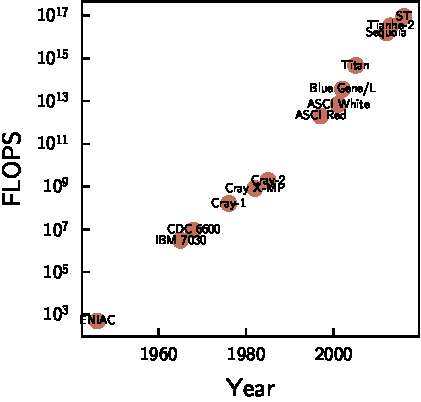
\includegraphics[width=1\linewidth]{./figures/supercomputer_flops.pdf}
		\caption{Number of Floating points operations evolution for the biggest supercomputer \label{fig:supercomputer_flops}}
	\end{figure}

	\section{Invariant Measures and Ergodicity}

    In statistical physics, the concept of an invariant measure plays a crucial role in understanding the long-term behavior of dynamical systems, and the symetry of the system (Noether's theorem). One of the main goals of computational statistical physics is to find algorithms preserving the invariant measure of the systems we are studying. For example we will see that the Euler algorithm is not a good choice for simulating Hamiltonian systems, as it does not conserve the energy of the system, as opposed to the Verlet algorithm, which is based on clever considerations of the symplectic\footnote{Symplectic geometry has its origins in the Hamiltonian formulation of classical mechanics where the phase space of certain classical systems takes on the structure of a symplectic manifold}.
	Ergodicity is another important concept in statistical physics, which ensures that the system explores the entire phase space in the long run. Which results in one of the most important hypothesis in computational statistical physics, the ergodic hypothesis, which states that the time average of a system is equal to its ensemble average.

	\chapter{Molecular Dynamics}
	\section{Hamiltonian Dynamics}
	\subsection{Hamiltonian Formalism}

	The Legendre transformation of the Lagrangian allows us to define the Hamiltonian of a system, which is a function of the generalized coordinates $q_i$ and the generalized momenta $p_i$ of the system (see CITE). The Hamiltonian is defined as :
	$$ H \defeq \frac{\textbf{p} ^T \textbf{M} ^{-1} \textbf{p}  }{2} + U(q)$$
	with $U(q)$ the potential energy of the system and $\textbf{M}$ the mass matrix of the system. The equations of motions can then be written using the Euler-Lagrange equations :
	$$
		\begin{cases}
			\dot{q} = \frac{\partial H}{\partial p} \\
			\dot{p} = -\frac{\partial H}{\partial q}
		\end{cases}
	$$

	This can be written in a more compact matrix form :

	$$ \begin{pmatrix}
			\dot{\textbf{q} } \\
			\dot{\textbf{p} }
		\end{pmatrix} = \textbf{J} \nabla H(\textbf{p} ,\textbf{q} )
	$$
	with $$\textbf{J} = \begin{pmatrix}
			0          & \textbf{I} \\
			\textbf{I} & 0
		\end{pmatrix} $$
	These type of non linear equations can only be ensured locally, but since the systems are Hamiltonian we can unearth the global existence and uniqueness of the solutions. Indeed we just need to show that using the energy constraints of the system the solutions are bounded for all time. For the impulsion this is trivial considering a potential global minimum :

	$$ \frac{\textbf{p}^T \textbf{M} ^{-1} \textbf{p} }{2} \leq E_0 - U_{min}$$

	For the position we just need an assumption on the level sets of the potential energy. $$ \Sigma_{\alpha} = {\textbf{q}|U(\textbf{q} = \alpha) }$$
	If these levels are bounded then the solutions are bounded for all time. This is not the case for all potentials, this is why for solving this kind of equations we will add sometimes confining potentials to the system.
	\subsection{Map Flow}

	Since the Hamiltonian equations are solvable, it seems natural to define a map flow $\mathcal{F}$ such that for an initial condition $z_0$ and a considered point $z_t$ we have :
	$$\textbf{z} _t = \mathcal{F}_t(\textbf{z}_0)$$
	This flow map is obviously invertible and Hamiltonian conservative. The key of numerical integration is then to approximate the true flow map of the system by the numerical flow map $\mathcal{T}$ such that the physical properties of the system are conserved over time.

	Considering the linear system for the differentiation :

	\begin{equation}
		\label{eq:linear_system}
		\dv{\textbf{z}}{t} = f(\textbf{z} ) = A\textbf{z}
	\end{equation}

	One way to solve this equation is to use the matrix exponential :

	$$\textbf{z}_t = \exp(At)\textbf{z}_0$$

	Then it appears that the flow map is given by :
	\begin{equation}
		\label{eq:flow_map}
		\mathcal{F}_t(\textbf{z} ) = \exp(tA)\textbf{z}
	\end{equation}

	\subsection{Sympletic Form}

	\subsubsection{Volume Preservation}
	One of the most important properties of the flow map is the preservation of the volume in the phase space. Indeed,for a Hamiltonian system we have thanks to Liouville's theorem the volume of a given sets of solution governed by \ref{eq:linear_system} is preserved over time if $$ \nabla \cdot f = 0 \, .$$

	It is easy to show that for a Hamiltonian system : $$\nabla \cdot f = \nabla \cdot \begin{pmatrix}
			0          & \textbf{I} \\
			\textbf{I} & 0
		\end{pmatrix} \nabla H = 0$$
	Due to the $\mathcal{C}^2$ property of the Hamiltonian. The main consequence of this property is that the flow map is volume preserving (Liouville Theorem), which has to be an important concern while building an integration algorithm to approximate the flow map.

	\begin{figure}[H]
		\def\svgwidth{\linewidth}
		\input{./figures/Phi_space_volume.pdf_tex}
		\caption{Volume conservation for the true Hamiltonian in black and the approximated Hamiltonian in red}
		\vspace{0.15cm}
	\end{figure}

	\subsubsection{Sympletic Property}
	The sympletic property of the flow map is another important characteristic of the Hamiltonian system. Indeed, the sympletic property of the flow map is defined as :
	\begin{equation}
    \mathcal{F}_t^T J \mathcal{F}_t = J
	   \label{eq:Sympletic}
	\end{equation}
With $J = \begin{pmatrix}
			0           & \textbf{I} \\
			-\textbf{I} & 0
		\end{pmatrix}$
        the sympletic matrix. This property leads to the conservation of the volume of the phase space, indeed one can easily show using (\ref{eq:Sympletic}) that we have  for the Jacobian associated with the map : $\lvert \mathcal{F'}_t\rvert^2 = 1 $.

        One interesting point of symplectic maps is that they form a group (they preserved the composition) which can be used to build other more complex symplectic maps. For example to increase the order of sympletic integrators $\mathcal{G}_h$  approximating the flow map $\mathcal{F}_h$, we can compose this latter with an other interesting sympletic integrator, this final integrator will then be sympletic and volume conservative. We can also split the integrator in two sympletic part if they are independant which is the case for Hamiltonian flow map in a pure potential $V(\textbf{q})$. This is called the splitting method \cite{MD_theo}, and will be the object of the next discussion.

	\subsection{Error Analysis for Hamiltonian splitting}

	\subsubsection{Lie Derivatives and Poisson Brackets}

	\paragraph*{Lie Derivatives}

	In the case of a non-Linear Hamiltonian system, the flow map can be approximated by the Lie derivative of the Hamiltonian, we would like to find again the convenient results :

	$$ \mathcal{F}_t = \exp(tA)\textbf{z}$$

	Let's consider a functional $\Phi$ of the phase space, the Lie derivative of $\Phi$ is defined as :

	$$ \mathcal{L}_f \Phi = \nabla \Phi \cdot f$$

	This is a generalization of the directional derivative to the phase space. Expanding the $\Phi$ map in a Taylor series we have :

	\begin{align*}
		\\ \Phi(\textbf{z}(t)) &= \sum_i \frac{t^i}{i!}(\mathcal{L}_f^i \Phi)( \Phi(\textbf{0} ))
		\\ &= \exp(t\mathcal{L}_f)(\Phi(\textbf{0}) )
	\end{align*}

	Applying this along the trajectory gives us the following map :

	$$\mathcal{F}_t(\textbf{z} ) = \exp(t\mathcal{L}_f)(\textbf{z})$$

	\paragraph*{Poisson Brackets}

	A common notation introduced in Hamiltonian mechanics is the Poisson bracket, which is defined as :

	\begin{align*}
		\\ \{g_1, g_2 \} &= \sum_{i = 1}^N (\pdv{g_1}{q_i}\pdv{g_2}{p_i} - \pdv{g_2}{q_i}\pdv{g_1}{p_i})
		\\ &= \nabla g_1^T \textbf{J} \nabla g_2
	\end{align*}

	Considering a smoooth scalar value function $F$ of the phase space, we can show that the Lie derivative of $F$ is given by the Poisson bracket of $F$ and the Hamiltonian :
\begin{equation}
    \mathcal{L}_{\textbf{J} \nabla H} F = \mathcal{L}_H F = \{F, H\}
    \label{eq:Lie_Hamiltonian}
\end{equation}

	Poisson brackets can be related to the Lie derivating noticing that for every real valued function $f$: $$[\mathcal{L}_{H_1}, \mathcal{L}_{H_2}]f = \mathcal{L}_{\{H_1, H_2\}}f$$

	\subsubsection{Error Analysis for non Commuting Hamiltonian}
    The main idea behinds this study is to consider integration method as a splitting of the Hamiltonian into several parts oftenly independant of one of the two system of coordinates $(\textbf{q}, \textbf{p})$, as we will see further. The poisson brackets are linear with respect to the Hamiltonian (\ref{eq:Lie_Hamiltonian}), which allows us to write the following considering $H = H_1 + H_2$,

	$$\mathcal{L}_H = \mathcal{L}_{H_1} + \mathcal{L}_{H_2}$$

	The flow map of the system is then defined as : $\mathcal{F}_t(\textbf{z}) = e^{t()\mathcal{L}_{H_1} + \mathcal{L}_{H_2})}\textbf{z}  $

	The splitting method has the following flow map : $$\mathcal{G}_th= e^{h\mathcal{L}_{H_1}}e^{h\mathcal{L}_{H_2}}$$ Which is not the same as the true flow map. To evaluate the error done considering the splitted Hamiltonian, we can use the Baker-Campbell-Hausdorff formula and the correspondance between the Lie derivative and the Poisson bracket unearthing :

	$$ e^{h\mathcal{L}_{H_1}}e^{h\mathcal{L}_{H_2}} = e^{ h \mathcal{L}_{\tilde{H}_h}}$$

    With $\tilde{H}_h$ the so called \textit{shadow Hamiltonian} \cite{MD_theo} :
    \begin{equation}
	\begin{split}
        &\tilde{H}_h = H_1 + H_2 + \frac{h}{2}\{H_1 , H_2 \} \\ 
        &+ \frac{h^2}{12}(\{H_1 \{H_1 , H_2\} \} - \{H_2 \{H_1 , H_2 \} \}) \\
        &+ \dots
	\end{split}
    \label{eq:shadow_H}
    \end{equation}

	From this we can easily understand that as long as the two split Hamiltonian do not commute, we have at least a linear error (one example is the sympletic Euler Method). One way to do that, is to find a split with commutating Hamiltonian, or to split $H$ into three Hamiltonian such that that the linear term vanishes when we develop the expansion (such as the Velvet Velovity \& position method). The main idea behind this  development was to show that the flow map $\mathcal{F}_t$ we approximate using the other $\mathcal{G}_t$ stands in the splitting method for an exact solution to an other (but similar) Hamiltonian system.

	To put in a nutshell the splitting method allows us to build sympletic integrator using Hamiltonian transformations. Not all interesting integrators have sympletic structures, but they should all have volume conservation properties at least on long time scales.
	\section{Time Integration}

	Here we will restrict our study to simple linear system. To perform time integration, we discretize time into small intervals $\delta t$ . At each time step $t_{n+1}=n \delta t$, we approximate the change in the system using matrix iteration.
	$$ \begin{pmatrix}
			x(n\delta t) \\
			y(n\delta t)
		\end{pmatrix} = \mathcal{T}^n(\delta t) \begin{pmatrix}
			x(0) \\
			y(0)
		\end{pmatrix}$$

	The goal is then to find the correct matrix such that iterating over time will not change the invariance of the system. To fit the previous notations the flow map can be defined as :
	$$\mathcal{F}_{\delta t}(\textbf{z} ) = T(\delta t)\textbf{z} $$ with $\mathcal{F}_{\delta t}$ a volume conservatuve flow map.

	\subsection{Application to the Harmonic Oscillator}
    The Harmonic oscillator is a simple system with a known solution, despite its simplicity it unearthed so key concerns for time integration algorithms (stability of the integrator, pseudo-conservation of the energy, etc.).
	$$\ddot{x} - \omega^2 x = 0$$
	\subsubsection{Exact Propagator}
    The exact time evolution of the system for a time translation of $\delta t$is given by the following propagator : 

	$$ \begin{pmatrix}
			x(\delta t) \\
			\dot{x}(\delta  t)
		\end{pmatrix} = \mathcal{T}(\delta t) \begin{pmatrix}
			x(0) \\
			\dot{x}(0)
		\end{pmatrix}$$
	With $$\mathcal{T}(\delta t) =  \left(\begin{array}{cc}
				\cos(wt)    & \frac{1}{w}\sin(wt) \\
				\-w\sin(wt) & \cos(wt)
			\end{array}\right)$$

	In the next analysis we will use a dimensionless time $\tau = \omega t$,  a dimensionless position $\xi = \sqrt{\frac{k}{k_BT}x}$ and a dimensionless impulsion $\Pi = \sqrt{\frac{1}{mk_bT}}p$ , which leads to the following time Propagator :
	\begin{align*}
		\\ \mathcal{F}_{\delta \tau} = \mathcal{T}(\delta \tau) &=  \left(\begin{array}{cc}
				\cos(\delta \tau)   & \sin(\delta \tau) \\
				- \sin(\delta \tau) & \cos(\delta \tau)
			\end{array}
		\right)
		\\ &=  \exp(\textbf{J} \delta \tau)
	\end{align*}

	Here we related as did previously the flow map to the derivative operation for our system.
	For the Hamiltonian we recover :

	$$ H = \frac{\mathcal{H}}{k_BT} = \frac{1}{2}(\Pi^2 + \xi^2)$$ Then let's consider a microstate of the system $\ket{\tau} = \begin{pmatrix}
			\xi(\tau) \\
			\Pi(\tau)
		\end{pmatrix}$
	The time evolution of the system is given by the following equation :
	$$ \ket{\tau + \delta \tau} = \mathcal{T}(\delta \tau) \ket{\tau}$$
	With the unitary propagation matrix $$\mathcal{T}(\delta \tau) = \begin{pmatrix}
			\cos(\delta \tau)         & \frac{1}{\omega}\sin(\delta \tau) \\
			-\omega \sin(\delta \tau) & \cos(\delta \tau)
		\end{pmatrix}$$
	Solving the characteristic equation $\lVert \mathcal{T} - \lambda I\rvert = 0$, we unearth the eigenvalues.
	$$ \lambda_\pm = \exp(\pm i \delta \tau), $$

	Considering the two \textbf{orthogonal}  eigenvectors $\ket{\pm}$, we easily show that :
	\begin{align*}
		\ket{n \delta t} & = \mathcal{T}(\delta t)^n \ket{0}                   \\
		                 & = a_+ \lambda_+^n \ket{+} + a_- \lambda_-^n \ket{-} \\
	\end{align*}

	Considering the initial decomposition $$ \ket{0} = a_+ \ket{+} + a_- \ket{-}$$

	Then we can easily show that :

	\begin{align*}
		\\ \frac{E}{k_bT} &= \frac{1}{2}\braket{n \delta \tau}{n \delta \tau}
		\\ &=\frac{1}{2}\left(\lvert a_+ \rvert^2  + \lvert a_- \rvert^2 \right)\mathcal{T}(\delta t)^n
		\\ &= \frac{1}{2} \braket{0}{0}
	\end{align*}

	Which shows that the energy is conserved over time. We can also show an interesting result about the conserved quantities : Every conserved property of the system is proportional to the Hamiltonian. 



	\begin{align*}
		\\ \expval{A}{0} &=\expval{A}{\tau}
		\\  & \Rightarrow A \equiv \mathcal{T}^\dagger A \mathcal{T}
		\\ & \Rightarrow A \propto H
	\end{align*}
    
	\subsubsection{Euler Algorithm \& Propagator}

	The Euler algorithm is the simplest algorithm to perform time integration, based on the first order approximation in Taylor expansion. The explicit non sympletic Euler algorithm is given by the following flow map :

	$$\mathcal{G}_{\delta \tau}^{\text{euler}} = I - S \delta \tau $$ With $S$ verifying $$\dv{\textbf{z} }{\tau} = S \textbf{z} $$ One can remark that for volume conservation the map should verify the following property : 
    \begin{equation}
        \det(I - S \delta \tau) =  0
        \label{eq:det_euler}
    \end{equation}

    Which is generally not the case in physical system were the eigen values of $S$ are in many cases,  pure imaginary. If we write the propagation matrix for the Euler algorithm, we obtain the following :

	$$ \mathcal{T}(\delta \tau) =
		\begin{pmatrix}
			1                     & \delta \tau \\
			-\omega^2 \delta \tau & 1
		\end{pmatrix}
	$$

	Which is not unitary, and not time reversible. We can show that the energy of the system is not conserved over time, through the same reasoning as before. Indeed, the two eigenvalues of the matrix are :

	$$ \lambda_\pm = 1 \pm i \delta \tau$$

	Which leads to divergence of the energy with the following expression :

	\begin{align*}
		H & = \frac{1}{2}\braket{0}{0}(1 + \delta \tau^2)^n          \\
		  & = \frac{1}{2}\braket{0}{0}\exp(n \ln(1 + \delta \tau^2))
		\\
	\end{align*}

    This divergence of the system can be seen in fig \ref{fig:Velevet_euler}. This lack of stability is closely related to the relation (\ref{eq:det_euler}), but stability analysis is a more complex subject, which will not be discussed here (see \cite{MD_theo} for more information).

	\subsubsection{Verlet Algorithm \& Propagator}

    The Verlet algorithm is a second-order algorithm, which is based on the symplectic structure of the phase space and directly derived from the splitting method. The point is to split the Hamiltonian into two parts, one depending only on the position and the other only on the impulsion. $$H = H_q + H_p$$ With $H_q = U(q)$ and $H(p) = \frac{p^TM^{-1}p}{2}$. If we just do that it is obviously from the shadow Expansion of the Hamiltonian (\ref{eq:shadow_H}) an order one method (the Euler sympletic method). For the velvet algorithm we want that the order one term vanishes, which leads to the following splits:

	$$H = H_1 + H_2 + H_3$$

	With the following possibility :

	$$\begin{cases*}
			H_1 = H_3 = \frac{1}{4}p^TM^{-1}p \quad|\quad H_2 = U(q)             \\
			H_1 = H_3 = \frac{1}{2}U(q) \quad|\quad  H_2 = \frac{1}{2}p^TM^{-1}p \\
		\end{cases*}
	$$
	One can show that the first order term vanishes in the shadow Hamiltonian, which defined a second order method. The first split is called the \textbf{position Verlet algorithm} , and the second the \textbf{velocity Verlet algorithm} . Let's focus on the velocity algorithm, this split is equivalent to the following canonical change of variable :

	\begin{align}
		\hat{\textbf{P} } & = \textbf{P}  - \frac{h}{2} \nabla U(\textbf{q} )         \\
		\textbf{Q}        & = \textbf{q}  +  \frac{h}{2}\textbf{p} ^TM^{-1}\textbf{p} \\
		\textbf{P}        & = \hat{\textbf{P} } - \frac{h}{2} \nabla U(\textbf{Q} )
	\end{align}

	This consist in a first drift $\frac{h}{2} \nabla U(\textbf{q}$, following by a kick  $\frac{h}{2}\textbf{p} ^TM^{-1}\textbf{p}$ and a final kick. This respect the hamiltonian srtucture of the system and gives the following  propagation matrix :

	$$
		\mathcal{T}(\delta \tau) = \begin{pmatrix}
			1 - \frac{\delta \tau^2}{2}                             & \delta \tau                 \\
			-\delta \tau \left(1 - \frac{1}{4} \delta \tau^2\right) & 1 - \frac{\delta \tau^2}{2}
		\end{pmatrix}
	$$

	Here we find an unitary matrix, which conserves a pseudo energy, but not the true Hamiltonian. This non conservation of the Hamiltonian is related to non orthogonality of eigenspaces, however we can still study the so called conserved pseudo energy and show that :
	\begin{align*}
		\expval{A}{0} & = \expval{A}{\tau}
		\\ & \Rightarrow A \equiv \mathcal{T}^\dagger A \mathcal{T}
		\\ & \Rightarrow A \propto \begin{pmatrix}
			1 & 0                                 \\
			0 & \frac{1}{(1 - \delta \tau^2/2)^2}
		\end{pmatrix}\underset{\delta \tau \rightarrow 0}{\longrightarrow} \propto H
	\end{align*}
	Hence, this time step dependent pseudo-energy converged to the wanted conserved value. This can be related to the discussion on the \textit{shadow} Hamiltonian, were we saw that the Hamiltonian describing the system in these kind of integration was changing, due to commutator terms. Hence, the true energy is not conserved but the energy corresponding to the exact description of the integration system is definitely conserved.
	\begin{figure}[H]
		\centering
		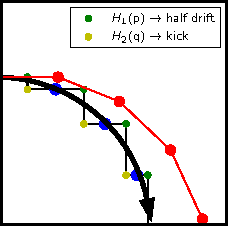
\includegraphics[width=1\linewidth]{./figures/Velvet_euler.pdf}
		\caption{\label{fig:Velevet_Construction} Here we compared the construction of the flow map for the euler and the velvet algorithm. We can see that for great time steps the Euler algorithm diverges from the true flow map, while the velvet algorithm stays close to the true flow map.}
	\end{figure}
	This is quite relevant to notice that for periodic system the euler algorithm is definitely not stable due to the non conservation of the volume. We can also see that as a consequence of taking the tangent for each time steps of the true flow map and will leads to exponential divergence from the trajectory in the phase space. This is why the velvet algorithm is a better choice for time integration of Hamiltonian systems.

    	\begin{figure}[H]
		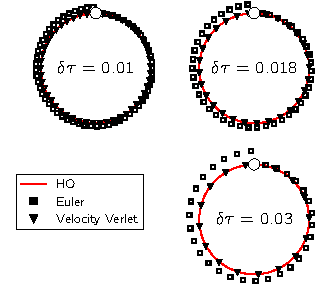
\includegraphics[width=1\linewidth]{./figures/HarmonicOscillator.pdf}
		\caption{\label{fig:Velevet_euler} To have a more general view of the efficiency of the integration scheme using a simple Harmonic oscillator we plotted the phase space trajectories for the Euler and the Velvet Algorithm, for two different timestep values}
	\end{figure}

	\chapter{Constant Temperature Dynamics}
	
    In molecular dynamics simulations, maintaining a constant temperature is essential for studying temperature-dependent properties and sampling the right thermodynamic ensemble. Various thermostats have been developed to control the temperature of the system, each with its own advantages and limitations. In this chapter, we will explore some common thermostats used in constant-temperature molecular dynamics simulations and discuss their properties.

    \section{Different Ensembles}

	In statistical physics, an ensemble is a large collection of hypothetical copies of a system, each representing a possible state that the system can be in. Ensembles are used to describe the macroscopic properties of systems based on the statistical behavior of their microscopic components. The concept of ensembles is fundamental in statistical mechanics because it allows the connection between microscopic interactions (the behavior of individual particles) and macroscopic observable (such as temperature, pressure, and magnetization).

    \subsection{Micro-canonical Ensemble}
    The micro-canonical set is the simplest ensemble in statistical mechanics, where the system is isolated and has a fixed energy. It is described using a constant number of particles $N$, volume $V$, and energy $E$. In an isolated system the fundamental postulates states that the system will explore all possible micro-states with the same probability. Hence we can define the density of micro-states for the micro-canonical ensemble as :

 $$ \rho_{\text{eq}} = \frac{1}{\Omega} $$

Where $ \Omega $ is the number of micro-states of the system with energy $E$,some key properties can be derived from this definition, such as the entropy of perfect gas, thermodynamic equilibrium pressure and chemical potential properties, but we will assume that known for the reader. The Micro-canonical ensemble is the one used when one simulate a physical system due to conservation laws regarding the Energy, however it is much more convenient to work with constant Temperature, for this we can introduce the canonical ensemble. 

\section{Canonical Ensemble}

\begin{figure}[H]
		\def\svgwidth{\linewidth}
        \input{./canonical.pdf_tex}
        \caption{Canonical ensemble schematic representation}
\end{figure}

In the Canonical ensemble we consider that our system is in contact with a biog reservoir, thus this two system composed a bigger isolated system. Then since the system $\mathcal{S} + \mathcal{R}$ is a microcanonical ensemble we get the following : 

$$ p_\mathcal{S} = \frac{\Omega_\mathcal{R}(E_\mathcal{R} =  E - E_\mathcal{S})}{\Omega_{\text{tot}}}$$
Considering the reservoir at equilibrium we get : 
$$\Omega_\mathcal{R}(E_\mathcal{R} =  E - E_\mathcal{S}) = \exp \left[ \frac{S_R}{k_B}(E - E_S)\right] $$
then if we develop the entropy around the mean energy of the system we get : 

$$ p_\mathcal{S} = \frac{1}{Z}\exp \left( - \frac{E_S}{k_B T_0}\right)$$

This stands for the Boltzmann-Gibbs distribution with $Z$ defining the partition function of the canonical ensemble and verifying the following relation : 
$$ Z = \sum_s \exp(-E_s / k_B T_0) $$.

A simple formulation of the partition function can be derived counting the degeneracy of the Energy level $\omega = e^{\mathcal{S}(e)/k_B}$. This will lead to the following expression : 

\begin{equation}
    Z = \int \exp(-\beta (E - T_0 \mathcal{S}(E))) dE
    \label{eq:partition_canonical}
\end{equation}

This motivates the definition of the free energy $F = E - T S$, and developing this latter around its minimum at the second order in the into grand gives the following : 

\begin{equation}
    Z = e^{-\beta (E^* - T_0 \mathcal{S}(E^*))}\sqrt{\frac{2\pi k_B}{- \pdv[2]{\mathcal{S}(E^*)}{E}}} 
    \label{eq:partition_canonical_2}
\end{equation}
This can be used to prove that the free energy is minimal at equilibrium in the thermodynamic limit. But here we will show that this imply a gaussian distribution of the energy.  Indeed using the previous calculation is leads to : 

$$ p(E) \propto e^{\frac{(E - E^*)^2}{2 k_B} \pdv[2]{\mathcal{S}(E^*)}{E}}$$
The study of the second moment then unearth : 
\begin{equation}
    \langle \Delta E^2 \rangle = - k_B \pdv[2]{\mathcal{S}(E^*)}{E} = k_B T_0^2C_V
    \label{eq:fluctuations_energy}
\end{equation}
With $C_V = \pdv{E}{T}_{(eq,N,V)}$ the heat capacity at fixed volume. This implied that the considering this latter at constant in a small range of temperature the energy distribution is a gaussian whose width is proportional to $T^2$.
\section{Thermostats}
This huge reservoir we used in the canonical ensemble is called a thermostat and is really convenient to dissipate external constraints apply on our system $\mathcal{S}$ while conserving a velocity in rough correspondence with temperature. This reservoir has to be able to exert forces and absorb energy from the system, this interaction can be defined in several ways from deterministic to stochastic method.
\subsection{Stochastic thermostat Thermostat}
\subsubsection{Andersen Thermostat}
The Andersen thermostat consists in refreshing the velocities of particles with a given probability at each timestep which $ P = v \delta t$ with the collision rate $v$. The refresh process is done by drawing a new velocity from the Boltzmann distribution at the given temperature, this can be done from scrambling or for every particles. This method is really simple and do not introduce concerns about ergodicity. However, despite the equation of motion being unchanged too high collision rate can dominate the underlying dynamics, slowing down the speed of exploring the phase space, and breaking the dynamics. Indeed it will leads to loss of memory and exponential decay of auto-correlation functions, while it is not the case in many MD systems.

In order to tackle this issue Andersen proposed $\nu \propto C_T \rho^{\frac{2}{3}}N^{-\frac{2}{3}}$ as a typical collision rate such that it should preserve the dynamics in most cases.
\subsubsection{Langevin Thermostat}
Changing the dynamics of the system 

The Langevin thermostat is a stochastic thermostat that introduces a friction term and a random force to the modified equations of motion. This thermostat mimics the effect of solvent particles collisions on the particles of the system (like the \textbf{Anderson} thermostat). The random force is a gaussian force whose amplitude is chosen independently from the dynamics but only on the Temperature of the system and the friction coefficient, so the more we damp the system the more we have to excitate it, this ensure that even tough we increase the damping effect the exploration of the phase space will not be too slow despite we broke the dynamics (as for the Andersen thermostat), on the other hand if we decrease the damping the exploration of the canonical distribution of energy will not be ensured.  The position Langevin equatiions in an harmonic potential in stationary state are given by : 
$$
\begin{cases} 
0 = \xi v(t) - kx(t) + f(t)\\
\langle f(t)f(t')\rangle = A \delta(t - t')\\
\langle f(t)\rangle = 0
\end{cases} 
$$

With the characteristic time $\tau = \xi/k$ and the friction coefficient $\xi$. The solution can be written as following : 

$$ x(t) = x_0 e^{-t/\tau} + \tau^{-1}\int_{0}^{t}e^{-(t - t') / \tau} f(t')dt'$$

\paragraph*{Amplitude of the noise}
And one can easily assert what we previously saw regarding the independence of the random force with the dynamics.
\begin{align*}
    \langle x(t)^2 \rangle &= A \xi^{-2} \int_{-\infty}^{t} e^{-2(t - t')/\tau}    \\                     
                           &= A \xi^{-2} \frac{\tau}{2} = \frac{k_B T}{k} 
\end{align*}
We then got the following : $A = 2 \xi k_B T $, this is a pretty interesting results since the noise amplitude is directly proportional to the friction constant (the more we damped the more we excite).
\paragraph*{Mean Square Displacement}
At very short time the $t$ the mean square displacement (\textbf{msd}) $\langle \delta r^2\rangle$ is only given by inertial effects (expending at the first order) and using the equi-partition theorem on the Kinetic energy, 

    $$\langle \delta r^2\rangle = d \frac{k_B T}{m}t^2$$
For longer timescales we have to study the effect of the friction term : 
\begin{align*}
  \langle \left( x_t - x_0\right)\rangle^2 &= 2 \left(\langle x^2 \rangle - \langle x_t x_0\rangle \right),\\
 &= 2\frac{k_B T}{\tau} \left(1 - e^{-t/\tau}\right)\\
\end{align*}
    this is done using the equi-partition theorem and : 
     $$\langle x_t x_0 \rangle = 2 \frac{k_B T}{\tau}e^{-t/ \tau} $$

For time $ t \ll \tau$ this leads to a diffusive process recovering the Enstein relation with the diffusion constant : 
 $ D = \frac{k_B T}{\xi}$, 

  $$\langle \left( x_t - x_0\right)\rangle^2  = 2Dt$$

  The $\tau$ constant is most of the time several order of magnitude above the characteristic time of the dynamics \cite{Correlation}. So we will generally considerate only the inertial and the diffusive regime


\begin{align}
    D &= \frac{1}{2}\lim_{t \rightarrow \infty} \dv{\delta r^2}{t} \label{eq:msd_grad}\\
    D &= \frac{\delta r^2}{2t} \label{eq:msd_diff}
\end{align}


One can note that the memory loss using the Langevin thermostat will be continuously impacted by the white noise, we used for sampling the canonical ensemble, leading to corrupted auto-correlation functions. To deal with that one can implement n memory term in the noise \cite{Correlation, MD_theo}, which has to be chosen carefully to not break the dynamics of the system. In addition this stochasticity break the continuous behavior of the system, and leads to discontinuity in average variables at least for andersen method.
\subsection{Deterministic Thermostat}

Studying the stochastic thermostats leads obviously to find and tweaks all the parameters such that we can preserve the physical behavior of the system, one can argue that we can use deterministic method to do the same sampling of the canonical ensemble, however these kind of methods generally lacks of ergodicity, and hardly reproduce the typical variation of the Kinetic Energy in the canonical ensemble [CITE].

\subsubsection{Velocity Rescaling}
The simplest way to obtain a constant temperature dynamics is to rescale the velocity by a factor :
\begin{equation}
    v'=\sqrt{\frac{K}{\mathcal{K}}}v 
    \label{eq:velocity_rescaling}
\end{equation}
With $K, \mathcal{K}$ respectively the total Kinetic energy and the desired Kinetic energy derived from the targeted temperature. 
Evans and Morriss (1983b) have shown that it leads to the following ensemble distribution  $p \left( \textbf{r}, \textbf{q} \right) $: 
\begin{equation}
    \label{eq:distribution_velocity_rescaling}
     \delta( K( \textbf{p}) - K_0) \delta( \textbf{P} - \textbf{P}_0 ) \exp \left( \frac{-V(\textbf{r})}{k_B T} \right) 
\end{equation}

With $\textbf{P}, K$ respectively the total momentum and kinetic energy. For the conformation probability distribution it is clearly the canonical one. For the momentum one,  it does not fit the canonical distribution. Which can lead to smaller oscillation in kinetic energy than the ones in the canonical ensemble. One can propose to add a specific timescale to relax the normalization which defines the Berendsen thermostat, where the velocity is this time slowing rescaled to the desired value : 

\begin{equation}
    \textbf{v}' = \textbf{v} \sqrt{1 + \frac{\delta t }{\tau}(\frac{K}{\mathcal{K}} - 1)}
    \label{eq:Berendsen thermostat}
\end{equation}

With $\tau$ the relaxation time, this method is really simple and can be used for equilibration, however it is not time reversible, and one can also show \cite{MD_theo} that it leads for vanishing $\tau$ to micro-canonical ensemble and isokinetic for diverging $\tau$. Rescaling the velocity seems to be a too strong constraint to sample correctly the canonical ensemble. On average, this will lead to the same results as canonical sampling since every ensemble is, in the thermodynamic limit, equivalents, however for fluctuations dependent observable this will exhibit wrong results.  These concerns were of strong interest in the 80's, leading to several (partial) solution. 

One way to solve this is to introduce a random velocity rescaling to mimic the fluctuations in the canonical ensemble, this can be done using the simple Velocity Rescaling (\ref{eq:velocity_rescaling}) or the Berendsen rescaling (\ref{eq:Berendsen thermostat}). To do so we just use a random pick for the Kinetic Energy drawn from the canonical distribution. 
$$ v' = \sqrt{\frac{\bar{K}}{\mathcal{K}}}, \quad \bar{K} \in $$
This is called \textbf{Canonical Velocity rescaling} (CVR), and as shown by (Bussi), under the assumption of ergodicity this sample correctly the canonical ensemble. One can argue that the dynamics can be altered, because of this stochasticity. 

An other totally deterministic approach is the Nose-Hoover formulation of the Dynamics.

\subsubsection{Nose-Hoover Thermostat}
The main idea here is to extend the system using two a new coordinate $s$ and a momentum $p_s$ representing the reservoir, the energy is then allowed to flow between the system and the reservoir. This leads to the following Hamiltonian of the total system :

$$\mathcal{H} = H(\textbf{p}, \textbf{r}) + \frac{p_s^2}{2Q} + gk_BT$$
With $Q$ the thermal inertia of the reservoir, $g$ the number of degree of freedom of the system. The choices of these parameter must me carefully done in order to ensure close coupling between thernmostating and dyncamics. The ensemble distribution is then :
$$\exp(\frac{-H(\textbf{q,p})}{k_BT}) \exp(\frac{-p_s^2}{2Qk_BT})$$
This beautifully stands for the canonical distribution in $\textbf{q,p}$. However Nosehimself found that this approach was difficultly exploring the phase for very simple system such as harmonic oscillator. Indeed, 
Nothing to drive the drive the fluctuations of $p_s$ [CITE] and fluctuations of the thermostating velocites are necessary to ensure the ergodicity of the system, since it will fill difficulty the phase space (coupling between the system and the reservoir). 
One possible solution is nose-hoover thermostatic chains, in order to drive the thermostat velocities with other reservoirs, this stands with the \textbf{CVR} as a perfect solution but Bussi argued we lost the beauty and the simplicity of the theory multiplying the thermostatic chain.

\begin{figure}[H]
    \begin{center}
        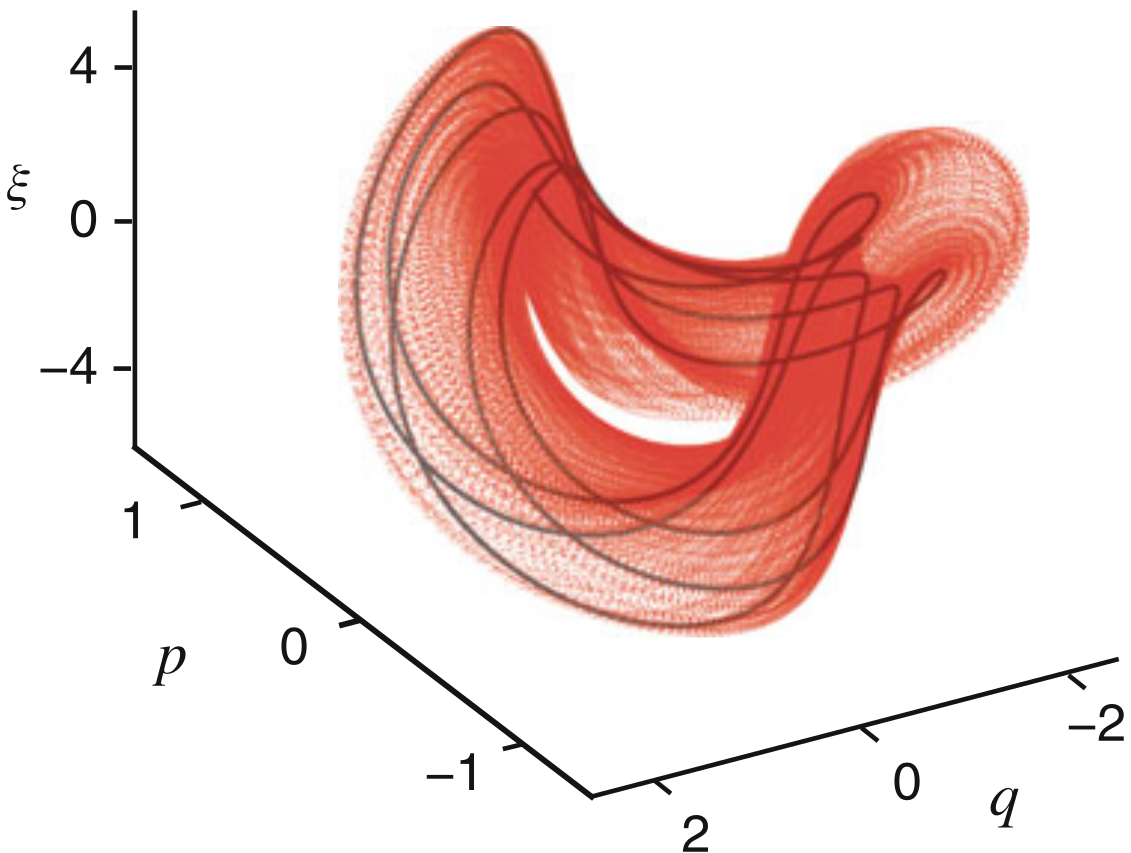
\includegraphics[width=1\linewidth]{./figures/NoseHooverChain.png}
    \end{center}
    \caption{length 2 Nose Hoover Chain applied on harmoic oscillator, trajectories are cought in an attractor, we do not recover the cannonical ensemble distribution (increase the number of chains [CITE], from [CITE]}\label{fig:NH-chain}
\end{figure}

\subsection{Comparing Thermostats}
Several studies can be done to compare the thermostat,the probability distribution function of the energy to see if it matches the canonical one, with high level of fluctuation. Regarding the dynamics we have to see if the velocity auto-correlation function is not dominated by thermostating effect, leading to corrupted transport coefficient calculation. 
\subsubsection{Energy Distribution}
Studying the impact of thermostating on the energy distribution is a simple way to see if you correctly sample the wanted ensemble without breaking the ergodicity or the dynamics of the system. 

Using (\ref{eq:fluctuations_energy}) we unearthed that the typical fluctuations of the energy in the canonical ensemble should be quite important, proportional to $T^2$. To ckeck which thermostat was able to mimic these fluctuations, we simulated a simple \textbf{LJ}-fluids with 32 particles equilibrated by different thermostats. The first step of the study was to calculate $C_V$ for this system, to do so we use the \textbf{CVR}, and showed that the heat capacity was remaining constant in the range of study. 
\begin{figure}[H]
    \begin{center}
        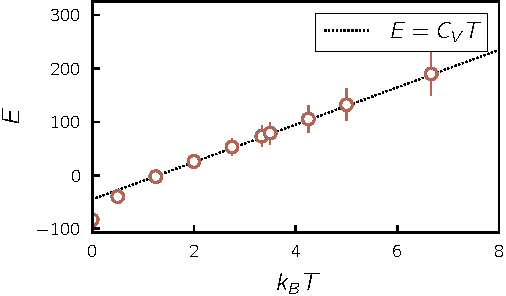
\includegraphics[width=1\linewidth]{figures/MD_energy_temperature.pdf}
    \end{center}
    \caption{Energy over Temperature, this plot unearths a value of Heat capacity at fixed volume : $C_V = 3.5e^1 \pm 1$}\label{fig:HC}
\end{figure}

Knowing that we can estimate the canonical distribution of the energy at second order using our previous study (\ref{eq:fluctuations_energy}).

$$ p(E) \propto e^{\frac{(E - E^*)^2}{2 k_B T_0^2 C_V}}$$

\begin{figure}[H]
    \begin{center}
        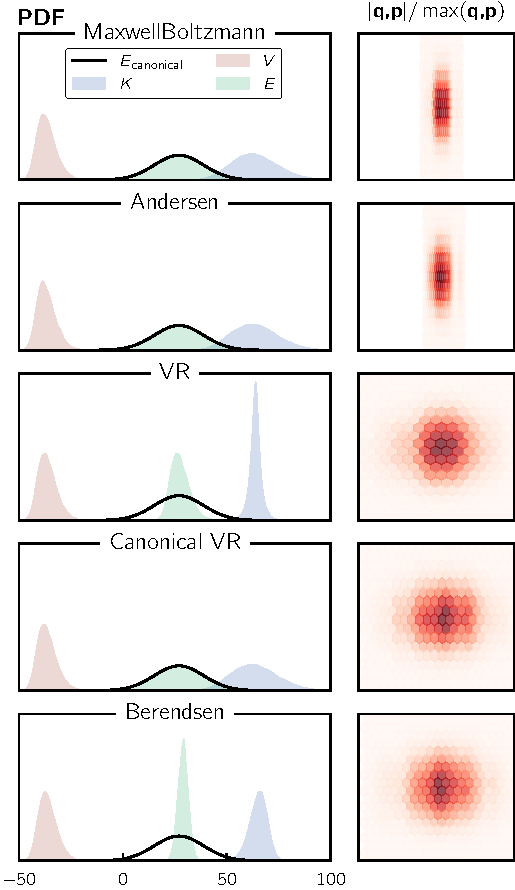
\includegraphics[width=1\linewidth]{figures/thermostats_PDF.pdf}
    \end{center}
    \caption{On the left we plots PDFs of potential $V$, kinetic $K$ and total energy $E$ for several thermostats. On the right we plot the normalized phase space hexbin histogram (in the sens of explorated domain size}\label{fig:PDF-th}
\end{figure}
 As intended the \textbf{Maxwell Boltzmann, Andersen, CVR} sample correctly the canonical distribution of energy, which appears normal considering their stochastic behavior. For the \textbf{VR, Berendsen} thermostat their non-canonical properties are clearly demonstrated with very small fluctuations of the Kinetic energy. However, one can notice on the fig \ref{fig:PDF-th} that the phase space exploration is inefficient for the \textbf{Maxwell-Boltzmann, Andersen} thermostat, with a very restricted exploration of the conformation space, this is mainly due to the fact that we broke the system dynamic, thermostating the velocities too often for this kind of thermostat. This issue does not appeared in the three other thermostats, where the phase space exploration is efficient.

 To put it in a nutshell thermostating is a subtle problem where we have to find the right equilibrium between sampling correctly the ensemble we want and the phase space in a reasonable time without breaking the dynamics, and ensuring ergodicity.

\subsection{Calculating Transport Coefficients}
To check if the thermostats preserve the physics of the system, we can study auto-correlations functions. Indeed referring to (Haile and Gupta, 1983), suitable thermostats should preserve the auto-correlations function of the velocity. It is simply a way of cheeking if the characteristic times of the system are unchanged. In addition to that a whole theory is dedicated to recover transport coefficient from auto-correlation functions (Green-Kubo relations). Here we will focus on the diffusion constant, which can be calculated from the velocity auto-correlation function (VACF).

\subsubsection{Long time tails}
In our simulated \textbf{LJ}-system the auto-correlation function of the system should decay slowly at large times, this is called long time tails phenomenon and is universal in this kind of fluid system. The first apparition of this result in the scientific litterature was back in the 70's witj the work of Alder and Wainwright simulating hard sphere. 

Indeed they unearthed a long time tailed of the form  $\sim t^{-\frac{d}{2}}$ 
contradicting the believed exponential decay of auto-correlation function (If we suppose that the dynamic follows the Langevin equation it is quite straightforward that it is the case). This dependancy was studied afterward by Pomeau and Résibois using long times hydrodynamics arguments. 

The main idea is rely on the local equilibrium implied by the presence of multiple particle fig.\ref{fig:long_time_tail}.b) these latter will interact between each other, leading to a constant velocity in a small volume $\Omega_t$ around the particle of interest, if you consider n particle interacting in this small volume then : 
 $$v(\tau) = v(0)/n \Omega_t$$
 This volume will spread with time fig.\ref{fig:long_time_tail}.c) dominated by hydrodynamic long time viscosity effect : $$\Omega_t = (\nu t)^{\frac{d}{2}}$$ with $d$ the dimension of the system. This leads to the following expression for the velocity auto-correlation function : 
 \begin{equation}
     v(\tau) \sim  v(0) \left( \frac{1}{\nu t} \right)^{\frac{d}{2}}     
    \label{eq:long_time_tail}
 \end{equation}
\begin{figure}[H]
		\def\svgwidth{\linewidth}
		\input{./decay_schema.pdf_tex}
        \caption{Schematics picturing the slow decay of auto-correlation functions, redraw from (Pomeau, Resibois \cite{POMEAU})}
        \vspace{0.15cm}
        \label{fig:long_time_tail}
\end{figure}

This dissipative spreading of the small volume $\Omega_t$ can be pictured by the following reasoning : considering a particle interacting in a repulsive way with others particles, this interaction will create an eddy behind the particle that will ensure that the particle continue in its original direction during a sufficiently long time. 
\paragraph*{Memory loss}
This slow memory loss is a key feature of the system, and can be used to check if the dynamics of the system is preserved by the thermostat. Indeed if the thermostat is too strong, the long time tail will be altered.
\begin{figure}[H]
    \begin{center}
        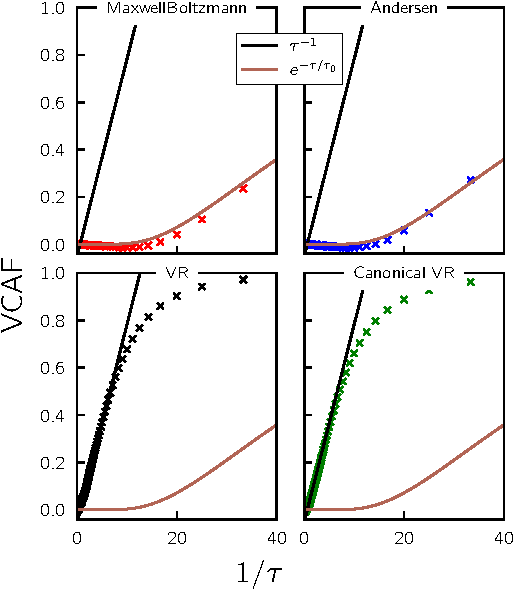
\includegraphics[width=1\linewidth]{figures/velocity_autocorrelation.pdf}
    \end{center}
    \caption{Normalized Velocity auto-correlation function}\label{fig:VCAF-th}
\end{figure}


\paragraph*{Dependance of the density}

To fall in this regime the system has to be dense enough as highlighted by \cite{density}. Indeed the long time tail is a collective effect, and will be more pronounced in dense system, where the particle are more likely to interact with each other and the vortex formation may not be sustained. To ckeck this behavior we simulated the same 2d system. Since the regime we studies should be dominated by collisions, we must know the time between the collision, the Enskog kinetic theory predicts : 

 \begin{equation}
    \tau_E  = \frac{1}{4 \rho \sigma^2 g(\sigma)} \sqrt{\frac{m}{\pi k_B T}}
    \label{eq:mean_time_collision}
 \end{equation}
 With $g(\sigma)$ the radial distribution function at the contact distance $\sigma$, this will be the characteristic length of the \textbf{LJ} potential in our case. For hard spheres it gives the following [CITE] : $$ g(\sigma) = \frac{1 - \pi \sigma^3 \rho / 12}{(1 - \pi \sigma^3 \rho / 6)^3}$$
We then decided to normalize the time by this time, and plot the VACF for different densities. Hence the density dependancy should not play a role anymore if it has only an effect on the collision time.
 \begin{figure}[H]
    \begin{center}
        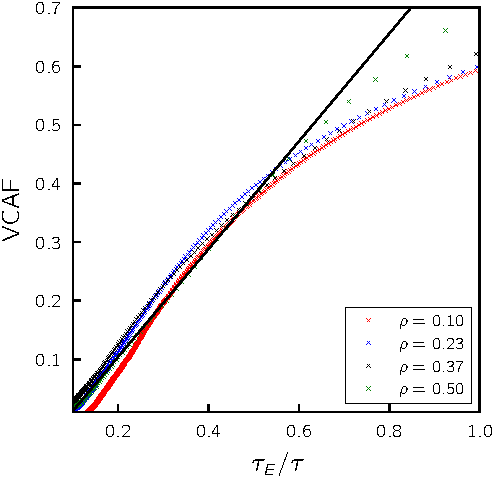
\includegraphics[width=1\linewidth]{figures/velocity_autocorrelation_density.pdf}
    \end{center}
    \caption{Normalized Velocity auto-correlation function over the approximated frequency of collision.}\label{fig:VCAF-thod}
\end{figure}
The density dependancy is not visible anymore except for very low or high collision frequency, and the \textbf{VACF} arounf the order of magnitude of the collision time is as expected comparable to $\sim \tau^{-1}$
\subsubsection{Calculation of Diffusion Constant}
The calculation of the velocity auto-correlation function is of great interest since it can be used to calculate the diffusion constant of the system, indeed we have : 

\begin{align*}
    D &= \lim_{t \rightarrow \infty} \frac{1}{2t} \langle \Delta r^2(t) \rangle \\
    &= \lim_{t \rightarrow \infty} \frac{1}{2t} \int_{0}^{t} \int_{0}^{t} dt'' dt' \langle v(t'' - t')v(0) \rangle \\
    &= \lim_{t_1 \rightarrow \infty} \frac{1}{2t} \int_{0}^{t} dt' \int_{0}^{t} dt'' \langle v(t'')v(0) \rangle \\
    &= \lim_{t \rightarrow \infty} \frac{1}{2t} \int_{-t}^{t} C(\tau) d \tau \int_{\max(- \tau,\tau)}^{\min(2t - \tau, 2t + \tau)} \frac{dv}{2}\\
    &= \lim_{t \rightarrow \infty} \int_{0}^{t} C(\tau) (1 - |\frac{\tau}{t}|)d \tau \\
    &= \int_{0}^{\infty} C(\tau) d \tau
\end{align*}
We lead this integration explecitely since it is rarely done in the literature, we used the following change of variable : 

 $$ \tau = t'' - t' , \quad v = t'' + t'$$
 The final expression is only valid when $C(\tau)$ decays faster than $\frac{1}{\tau}$ otherwise we got a logarithmic growth of the integral over time, this one of the numerically challenging issue when we focus on long time decay of the VACF, since we need to push the integration further, and run longer simulation. In 2d simulations we might even not be able to integrate because of the logarithmic growth of the integral. This way of calculation is commonly use but one should remember this integration subtility. With this latter  we now have three way of calculating the Diffusion coefficient, one can ask which one is the most reliable depending on the situation. M.P.Allen and D.J.Tidesley already discussed about it \cite{Correlation}, and drew the following conclusions. For exponential decay of the \textbf{VCAF}, it might be more accurate to compute gradient of the \textbf{msd} rather than dividing it by the time. So we will generally prefer (\ref{eq:msd_grad}) than (\ref{eq:msd_diff}). Regarding the calculation of the diffusion constant using the auto-correlation integration, we just need to integrate over the whole time to not miss long-time contributions. 

\begin{figure}[H]
    \begin{center}
        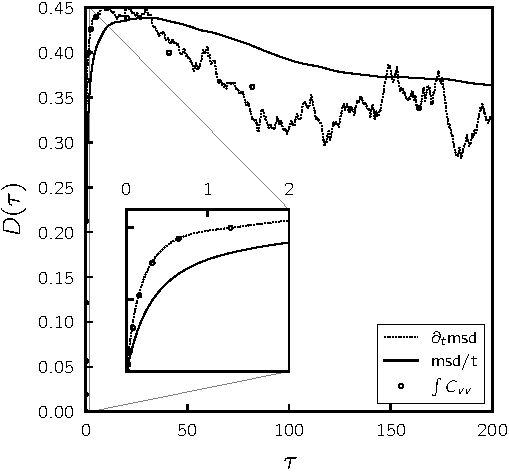
\includegraphics[width=1\linewidth]{figures/diffusion_calculation.pdf}
    \end{center}
    \caption{Diffusion coefficient over time using the previous described methods}\label{fig:diffusion-calculation}
\end{figure}

\chapter{Metropolis Algorithm}

\section{Monte Carlo Integration}
In Monte Carlo integration, we estimate an integral
\[
I = \int_{\Omega} f(x) \, d\mu(x)
\]
by averaging the function values at a set of randomly sampled points. If we sample \( N \) independent and identically distributed (i.i.d.) points \( x_1, x_2, \ldots, x_N \) uniformly over the domain \( \Omega \), the Monte Carlo estimate of the integral is given by:
\begin{align*}
    I &= V(\Omega) \langle f(x) \rangle_{\Omega} \\
    \hat{I}_N &= \frac{V(\Omega)}{N} \sum_{i=1}^N f(x_i). \\
\end{align*}

The Monte Carlo estimate is unbiased, meaning that the expected value of the estimate is equal to the true integral. But one can remark that the convergence is quite slow, indeed for the uniform sampling we evoked before it leads to the following variance of the estimator :

\begin{equation}
    \sigma^2(\hat{I}_N)= \frac{V(\Omega)^2}{N}\sigma^2(f(x))
    \label{eq:Variance}
\end{equation}
the error can then be estimated bu the standard deviation $\sigma$ which converges as $O(\frac{V}{\sqrt{N}})
$. This is quite promising since the error convergence rate is independent of the dimensionality which beats the "\emph{curse of dimensionality}". Indeed for a simple deterministic 2nd order Simson rule the convergence will in a space of dimension $d$ : $O(N^{2 / d})$, due to the number of evaluation we do. However one could not be satisfied by this poor convergence rate of $\frac{1}{2}$. Some solutions can be proposed as non-uniform sampling or important sampling. 


\section{Importance Sampling in Monte Carlo Simulations}

\textbf{Importance sampling} is a technique used in Monte Carlo simulations to improve the efficiency of sampling by reducing the variance of the estimator. The goal is to focus computational effort on regions of the state space that contribute most significantly to the density of states. However this sampling cannot be done without care and should respect some properties of the density of states such as its constancy at equilibrium.

\subsection{Concept of Detailed Balance and Equilibrium}

In statistical mechanics, \textbf{detailed balance} is a condition that ensures a system will reach and maintain equilibrium. It requires that, for any two states \( \nu \) and \( \mu \), the rate of transitions from \( \nu \) to \( \mu \) must equal the rate of transitions from \( \mu \) to \( \nu \) at equilibrium. Mathematically, this condition is written as:
\begin{equation}    
P(\nu) W(\nu \to \mu) = P(\mu) W(\mu \to \nu)
    \label{eq:random-walker}
\end{equation}
This ensures that  at equilibrium the probability distribution remains unchanged over time. This detailed balance properties, appears simple but restrict set of possible scheme Monte Carlo simulation.Indeed if we consider the following scheme for a Physics system, where we choose to do a move in the phase space dependind on the implied energy variation $\Delta E$ :

$$
\begin{cases}
    \text{If } \Delta E < 0, \text{ accept the move} \\
    \text{If } \Delta E > 0, \text{ reject the move} 
\end{cases}
$$

Since the scheme does not allow upward energy fluctuations (where \( \Delta E > 0 \)), the condition:
\[
P(\nu) W(\nu \to \mu) = P(\mu) W(\mu \to \nu)
\]
is not satisfied for all transitions. Here we understand that thermal fluctuations are crucial for the system to explore the entire configuration space properly. 
\subsection{Metropolis Algorithm}

To ensure that the Monte Carlo algorithm preserves detailed balance, transitions that increase energy must be allowed with appropriate probabilities most of the case it is given by the canonical ratio of the two state probabilities $p_{\mu}, p_{\nu}$). This is typically done using the \textbf{Metropolis algorithm}.
Indeed, The Metropolis criterion ensures that the detailed balance condition is satisfied because:
\[
\frac{W(\nu \to \mu)}{W(\mu \to \nu)} = \frac{P(\mu)}{P(\nu)} = \exp\left(-\frac{\Delta E}{k_B T}\right),
\]
where \( \Delta E \) is the energy difference between states \( \nu \) and \( \mu \). This allows the system to transition both to higher and lower energy states, maintaining the equilibrium distribution.

\section{Ising Model}
The Ising model is a fundamental model in statistical physics used to study phase transitions and critical phenomena.
\begin{figure}[H]
    \begin{center}
        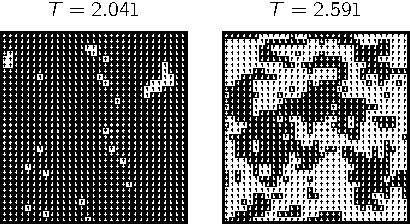
\includegraphics[width=1\linewidth]{figures/ising.pdf}
    \end{center}
    \caption{Two configurations of the same random walker (respectively for $T < T_C$ and $T>T_C$, with $T_C \approx 2.269$  using a $L = 32$ size periodic ising model}\label{fig:ising}
\end{figure}

 It consists of discrete spins arranged on a lattice, where each spin can point up or down and interacts only with its neighbors. Ising model is a really simple model that unearth some interesting physical behavior while studying phase transitions. 
\subsection{Theoritical Background}
The constant coupling ising model is defined by its Hamiltonian:

 $$ \mathcal{H} = -J \sum_{i,j} s_i s_j -B \sum_{i} s_i $$

Where \( s_i \) are the spins laying on a $d$ dimensional grid, \( J \) is the coupling constant, and \( B \) is the external magnetic field. This model has been solve exactly for dimension 1 and only without external magnetic field in dimension 2. Some simplifications can be made considering \textbf{Mean Field Approximation}, but these approximation leads to misleading behavior near the phase transitions with wrong critical exponent. Here we can define two important quantities, the spontaneous magnetization and the coupling term $M, Q$ :
    \begin{align*}
        M &=  \sum_{i} s_i \\
        Q &= \sum_{i,j} s_i s_j
    \end{align*}
Generally we study the reduced quantity $m, q$ with respectively : $m = \frac{M}{N}$ and $q = \frac{Q}{N}$
, we will also define the susceptibility $\chi = \pdv{m}{B}$. 
\paragraph*{Phase Transitions}
For the next discussion we will focus on thermodynamic limit, the system at stake will then be infinite. 
A phase transition occurs when a given quantity called the order parameter change from a zero value to a non zero value (for ferromagnetic system the order parameter is the spontaneous magnetization). Depending on the behavior of the system at the critical point one can define several type of phase transition.  


For first order transition first derivatives of the free energy are discontinuous at the
transition temperature. For the second order first derivatives are continuous. It will lead to metastable states or hysteresis phenomena in the first case and critical phenomena in the second case, with divergence of correlation length and time. In our case a 2nd order transition can be observed while sweeping the temperatures, and 1st order while seeping the external magnetic field for fixed temperature

Applying these definitions to our Ising model, we can unearth this two order of transition. 

\paragraph*{Magnetization discontinuity for first order transition}

For sufficiently low temperature, bellow the critical temperatures. One can find a first order transition for $B = 0$ while sweeping the external magnetic field $B$. The system will undergo an abrupt change from  a positive or negative magnetization depending on the starting state, for example if we start from a positive magnetization state we will go from $M_{sp}(B \to 0^+)$ to $-M_{sp}(B \to 0^-)$. We can illustrate that using the simple mean field approximation , we recall that this leads to the following expression : 

\begin{align}
    m = \tanh{\left( \frac{4Jm + B}{k_B T} \right)} \label{eq:magnetization-mean-field}\\
    \frac{k_BTx - B}{4J} = \tanh(x) \nonumber
\end{align}

With $ x = \frac{4Jm + B}{k_B T}$. This implicit equation can be solved graphically, for T bellow critical temperature ( $T_c = \frac{4J}{k_B}$, which is not the write value for the 2d ising model). For now we will limit ourselves to the following two case ($m< 0$, $B <0$) and ($m>0$, $B>0$).
\begin{figure}[H]
 \begin{tikzpicture}
 \begin{axis}[
legend pos=south east,
legend style={draw=none},
 variable = t,
 axis lines = middle, 
 xticklabel=\empty,
 yticklabel=\empty,
 ymin=-1.25, ymax=1.25,
xmin=-5, xmax=5,
 width=1.25\linewidth,
 height = 0.9\linewidth,]
\addplot [ domain=-5:5, samples=200, color=black,name path=A]{tanh(x)} ;
\addlegendentry{\scriptsize $\tanh{x}$}
\addplot [ domain=-5:5, samples=200, color=black,name path=B, densely dashed]{.4 * x - .2};
\addlegendentry{\scriptsize $\frac{k_B T x - B}{4J}$}
\draw[fill = black] (axis cs:0,-0.2) circle (.5pt) node[above,text=black] {};
\draw[-, color = black] (axis cs:0.3,-0.3) -- (axis cs:0,-0.2) node[below right,text=black] {\footnotesize $\frac{-B}{k_B T}$};
\draw[draw,name intersections={of=A and B, by={a,b,c}}, fill=black] 
        (a) circle (1pt) 
        (b) circle (1pt) 
        (c) circle (1pt);
    \draw[densely dotted, color = red] (a) -- (a |- {axis cs:0,0}) node[above,text=black] {\scriptsize{$x_0$}};
\draw[densely dotted, color = red] (b) -- (b |- {axis cs:0,0}) node[above,text=black] {\scriptsize $x_1$};
\draw[densely dotted, color = red] (c) -- (c |- {axis cs:0,0}) node[below,text=black] {\scriptsize $x_2$};
\node at (axis cs: -3, 1) {\scriptsize $T < T_c, \quad B >0$};
\node at (axis cs: 4.8,-.15) {\scriptsize $x$};
\end{axis}
 \end{tikzpicture}

\caption{Graphical resolution of the mean field equation (\ref{eq:magnetization-mean-field}) for $T < T_c$ and $B > 0$}
\end{figure}
If we limit to the case ($m>0, B>0$), only the $x_2$ solution is feasible since we got the following requirements $x > 0$, one can also suggest graphically that the $x_2$ value has an infimum independent from the magnetization and only dependent of the temperature since it's a solution of an implicit equation independent of m $x^+ > 0 $. This will lead in the limit of vanishing magnetic field starting from positive magnetization $$m^+ = x^+ k_BT$$ From the same reasoning we got similarly $$m^- = -x^+ k_BT$$ 
With this simple modeling we explain how the ising model can exhibit discontinuities in the order parameter and hence a first order transition, another cleaner proof can be done using fluctuation dissipation theorem \cite{Susceptibility}, exhibiting divergent behavior of the susceptibility at the transition point.

\begin{equation}
    \chi = \frac{N}{k_B T}( \langle m^2 \rangle - \langle m \rangle^2) \propto N
    \label{eq:Finite-sucepbility}
\end{equation}

Despite its usefulness this model present some limitations for this order of transiting, the mean field approximation consists in considering small fluctuations at the transition, this locality leads to meta stable states, that cannot exist in the 2d infinite ising model, since it is always at equilibrium. This metastables states arised from the $x_0, x_1$ solution and scales with the Coupling Constant of the system (see fig.\ref{fig:mfa}).

\begin{figure}[H]
    \begin{center}
        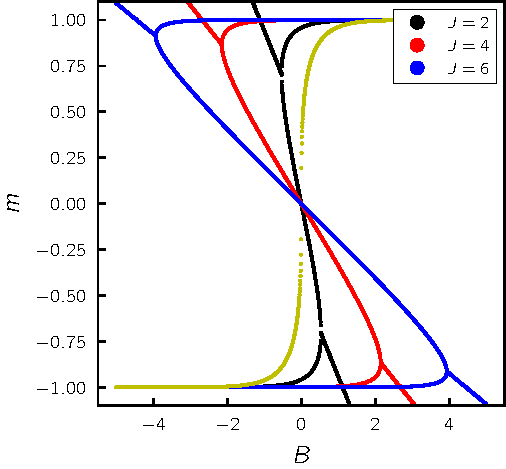
\includegraphics[width=1\linewidth]{figures/magnetization_mfa.pdf}
    \end{center}
    \caption{Magnetization Isotherm for several coupling constants, solved using approximation of the implicit equation}\label{fig:mfa}
\end{figure}

Here we see the characteristic hysteresis behavior of the first first order transition for the mean field apIsing model, and results from the locality of the approximation, highly correlated structure are then more resistant to change of the external magnetic field. 

\paragraph*{Critical behavior for Second Order Transition}

For second order transition, one can show that thermodynamic properties scales as power low of the reduced distance to the critical temperature $\epsilon = |1 - \frac{T}{T_c}|$.In the Ising model, Onsager unearthed that a second order transition is obtained for $B =0$, $\epsilon \to 0$. In this case we can express with this kind of power laws the order parameter $m$, the heat capacity $C_V$ and the magnetic susceptibility $\chi$, which respectively characterized how the system react to a change of Temperature and External Magnetic Field. The exponents of theses laws are called critical exponents and are usually constants for $T>T_C$ and $T < T_C$ (fore the amplitude of the power law this is not the case \cite{Landau}). for the magnetization it is more complicated in the ising case, since it should vanish infinitely fast  at 0, when $T  > T_c$. For example in the Ising model we got the following scaling laws when $ \epsilon \to 0$ \cite{power}. 

\begin{align*}
    m &\sim \epsilon^{\beta} &, \quad \beta &= \frac{1}{8} \\
    C_V &\sim \epsilon^{-\alpha} &, \quad  \alpha &= 0\\
    \xi &\sim \epsilon^{-\nu} &, \quad  \nu &= 1\\
    \chi &\sim \epsilon^{-\gamma} &, \quad  \gamma &= \frac{7}{4}\\ 
\end{align*}

With $m$ the magnetization, $C_V$ the heat capacity, $\xi$ the correlation length and $\chi$ the magnetic susceptibility. These critical exponents are universal, meaning that they are independent of the microscopic details of the system. 

\subsubsection{Finite Size Effect}
Since we cannot simulate an infinite system, we have to restrict to finite system where the thermodynamic limit is not ensured anymore, for this study we will not consider boundary effect that can play an important role at the critical point \cite{Landau}.

Finitness of a system lead to important change in the critical behavior, indeed the thermodynamic properties are smoothed and do not diverge near the transition point \cite{Landau}, and the order parameter change continuously during the transition,  this might lead to difficulty distinguishing 1st and  2nd order transition. For second order transition in finite system the correlation length cannot diverge (as in first order transition) because it is obviously limited by the system size $L$. 

For first order transition the discontinuity of the magnetization is smeared out by the finite susceptibility, leading to a continuous variation of the magnetization while sweeping $B$ contradicting our previous study. 

\paragraph*{First Order Transition in Finite Size System}
Here we will consider the most interesting case for finite size i.e $T< T_c$. In these conditions the system will undergo a smooth change of magnetization, and one could unearth some metastable state due to the locality implied by the finite size. Indeed even if we let the system equilibrate it will be trapped in these local minima of free energy due to predominance of surface effect. In addition to that the susceptibility is no more spiking for equilibrium state (as we saw previously) \cite{Susceptibility}. Indeed due, to finitness the susceptibility is bounded and evolves proportionally to the system size (eq.\ref{eq:Finite-sucepbility}), explaining the smooth change of the magnetization (see fig.\ref{fig:1st-finite}).  

\begin{figure}[H]
    \begin{center}
        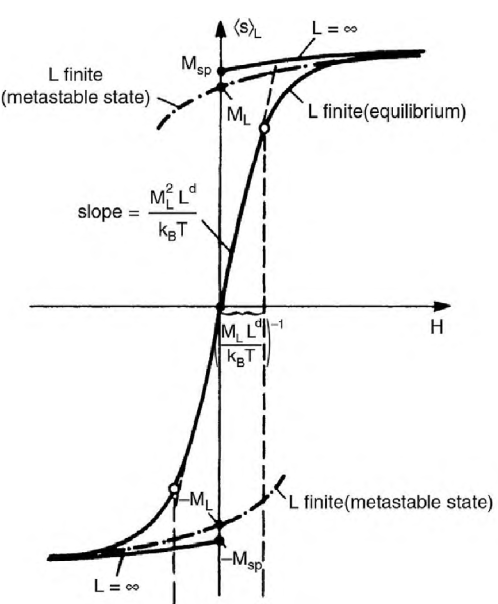
\includegraphics[width=1\linewidth]{figures/first_order_finite.png}
    \end{center}
    \caption{Variation of the magnetization in a finite Ising model, $M_{sp}$ denotes the magnetization at for the infinite phase transition, $M_L$ for the finite one, from (Landau, David P. and Binder, Kurt, 2014) \cite{Landau}}.
        \label{fig:1st-finite}
\end{figure}

The system will then jumped back and forth between the two minimum of the free energy, leading to a unevenly weighted bimodal distribution of the magnetization (see fig.\ref{fig:hysteresis-loop}). The existence of metastable states results in hysteresis loop depending on the starting configuration. Hence we can see that determining the critical point can be really hard knowing this hysteresis phenomenons, since it is constantly shifted by the existence of metastable states whose weight is dependent on the system size and the simulations parameters.

This bahavior had been studied in the fig.\ref{fig:hysteresis-loop}. Where the characteristic bimodal distribution appeared, the width size dependancy shows correct agreement with \cite{Landau}, with narrower distribution for higher $L$. The size dependant slope is also clearly visible, denoting finite susceptibility at the transition point $\propto N$. In our study the hysteresis behavior has only been found for $T < T_C$ as opposed to \cite{PhysRevE.52.1399} where they used sinusoidal driving. The number of sweeps we used for Monte carlo simulations does not seem to play a great role contradicting at first sight the results of \cite{PhysRevE.52.1399}, but here they used logarihmic valued of the sweeping parameter, this can lead to very fast exploration of the phase space but also to issues in the equilibration of the walkers. The simulation temperature has interesting impacts on the hysteresis behavior. Indeed, increasing the temperatures seems to decrease the hysteresis effect, while reducing the population in the metastable states.

\end{multicols}
\par\noindent\rule{\textwidth}{0.4pt}
\begin{figure}[H]
\begin{center}
        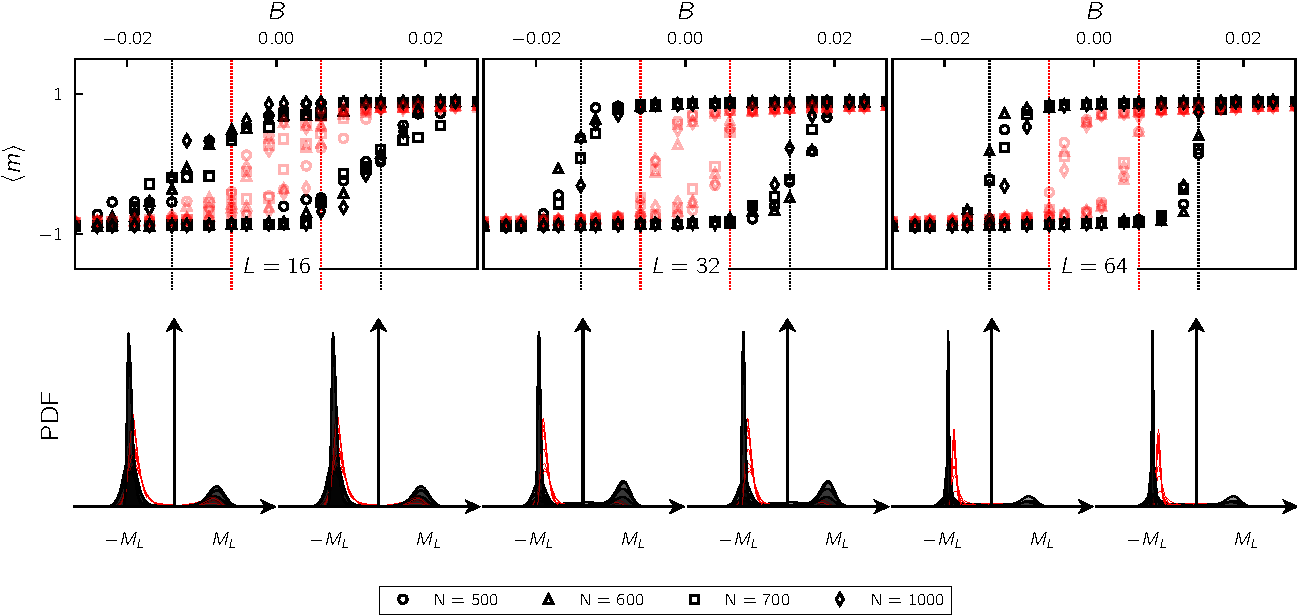
\includegraphics[width=1\linewidth]{figures/Ising2D_1st_order_transition.pdf}
    \end{center}
    \caption{On the top row, we plot the magnetization evolution while seeping the magnetic field $B$ for different system size. The bottom row shows the corresponding histogram of the magnetization for $T = 2$ and several Monte Carlo sweeps (N). Red transparent dots stands for simulations done near the critical point $T = 2.269$, and black solid dot correspond to $T = 2 < T_C$.  To get this clear metastability we started with negative $B$ for \texttt{all-down-state}, and with positive $B$ for \texttt{all-up-state}, then we increased and decreased respectively the magnetic field until we reach the opposite conformation. The sweeping frequency study has been motivated by \cite{PhysRevE.52.1399} where it is shown that the magnetic sweeeping rate has a strong impact on the hysteresis below and above $T_C$}
    \label{fig:hysteresis-loop}
\end{figure}
\par\noindent\rule{\textwidth}{0.4pt}
\begin{multicols}{3}
In first order transition oner can show \cite{Landau} that the size of the system only play a role in the width and in the ampllitude of the distriubution with the same contribution a $L^d$ factor. One can then understand that smart rescaling can leads to correct infinte behavior of the simulation.

In 2nd order phase transition the thermodynamics are governed by critical power laws, so we expect this finite scaling to change. 
\paragraph*{Second Order Transition in Finite Size System}

It might seem more difficult to extract inifinte behavior for this kind of power laws. However one is able quite straightforwardly to extract infinite behavior from finite size simulations considering finite size scaling of the free energy \cite{Landau} (this express the dependancy of the free energy over the length of the system in a simple way). Differentiation of this latter yields the following scaling laws for the order parameter and the susceptibility. 

\begin{align}
    m_L &= L^{-\beta/\nu} \mathcal{M}_0(\epsilon L^{\frac{1}{\nu}})\\
    \chi_L &=L^{\gamma/\nu} \chi_0(\epsilon L^{\frac{1}{\nu}})
\end{align}

Where $\mathcal{M}_0$, and $\chi_0$ are scaling functions of the infinite system. Then we can easily propose to rescale the finite thermodynamics properties by the corresponding length dependencies, and to use the rescaled relative distance to the critical temperature $\epsilon L^{\frac{1}{\nu}}$. For example here we studied the rescaled susceptibility and magnetization for different system size (see fig.\ref{fig:2n-order-scaling}). 

\begin{figure}[H]
    \begin{center}
        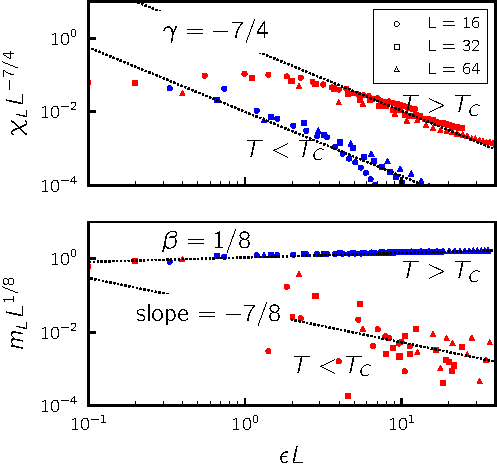
\includegraphics[width=1\linewidth]{figures/2nd_order_scaling.pdf}
    \end{center}
    \caption{Scaling laws for respectively the susceptibility and the magnetization for different system size. The simulations have been done using 10 random walkers with 500 checkboards sweep.}\label{fig:2n-order-scaling}
\end{figure}

First the curves collapse on a single one, proving the validity of these scaling laws over the finitness of the system. In addition to that we recover quite precisely the infinite scaling laws for the susceptibility and the magnetization. With the same slope for heating or cooling down the system for $\chi$. For the magnetization it seems to exhibit a $\frac{7}{8}$ critical exponents already discussed in \cite{Landau}.

\subsubsection{critical slowing down}
As we saw previously the correlation length is diverging when we reach $T_C$, long wavelength phenomena are then dominant. In this situation one can understand that local spin flip will not lead to correct sampling of the phase space since it does not allow to perturb the highly correlated system. For a constant observable  $A$, one can show (Hohenberg and Halperin, 1977) that the spatial components $\tilde{A}(q)$ of the Fourier transform $\tilde{A}$ follows the following relation : 

$$\tau_{AA} = (D_{AA}q^2)^{-1}$$

With $D_{AA}$ a transport coefficient. For example in spin exchange trial Move (Kawasaki), the concentration for each spin values is maintained constant. Hence for due to divergence of the correlation length the time to decorrelate the system will diverge as well, leading to a critical slowing down. To tackle this issues on can propose other trial move than just a local flip of one spin. The idea is then to flip larger domains of the system while preserving the flux of random walker (\ref{eq:random-walker}). This can be done using percolation method (Wolff cluster algorithm) to determine the spins to flip in a single move, in this case we can choose the percolation rate in order to always flip the selected cluster while preserving the flux, which leads to extremely fast exploration of the phase space. Checkboards methods can also be used to apply basic flip trial on all non neighboring spins without breaking the simulations. 


\section{Thermodynamic Integration}

Thermodynamic integration is a method used to compute the free energy. The major issue is the impossibility of sampling all the phase space in a simulations. Indeed the free energy is derived using the partition function of the ensemble 

 $$ F = -k_BT\log{Z}$$

The partition function is a sum over all the possible states of the system, and is then impossible to compute exactly. However, the exact value of the free energy is not necessary, since we are often interested in the relative free energy between two thermodynamic states. We can then use several method to directly or iteratively calculate this differences.

\subsection{Kirkwood Coupling Parameter}
The Kirkwood coupling parameter method provides a simple way to connect two states using a linear interpolation parameter \( \lambda \) between their Hamiltonians:
\[
H(\lambda) = (1 - \lambda) H_0 + \lambda H_1,
\]
where \( H_0 \) and \( H_1 \) are the Hamiltonian of the initial and final states. The derivative of \( H(\lambda) \) with respect to \( \lambda \) is given by:
\[
\frac{\partial H(\lambda)}{\partial \lambda} = H_1 - H_0.
\]

The Free energy has interesting properties related to the derivative of the Hamiltonian, indeed supposing the Hamiltonian can be written as a function of the coupling parameter $\lambda$, we can express 

$$\dv{F}{\lambda} = \langle \dv{H(\lambda)}{\lambda} \rangle_{\lambda}$$
Thus, the free energy difference between the two states $\ket{1}, \ket{2}$ is given by:
\[
\Delta F = \int_0^1 \left\langle H_1 - H_0 \right\rangle_{\lambda} \, d\lambda.
\]
\subsubsection{Mechanical and Thermodynamic Observable}
One can notice that we link the derivative of a global thermodynamic observable depending over the whole phase space to the derivative of a measurable mechanical observable $H$ defined for each specific state. This is the general the idea of the thermodynamic integration, linking the global thermodynamic properties to the local mechanical properties. 
\subsubsection{Ising Model case study}
In the Ising Model defined previsouly one can easily verify that : 
 $$
 \begin{cases*}
     \pdv{F}{B} = \langle M \rangle \\
     \pdv{F}{k} = - \langle Q \rangle
\end{cases*}
$$

Hence at first order for a small change of the magnetic field $B$ and the coupling constant $k$ we can easily compute the free energy difference between two states $(h_i, k_i)$, $(h_j, k_j)$ by expending $F$ around these two points. 
\begin{equation*}
\begin{split}
    \Delta F = &\frac{h_j - h_i}{2} (\langle M \rangle_i + \langle M \rangle_j)\\
    +&\frac{k_j- k_i}{2} (\langle Q \rangle_i + \langle Q \rangle_j)\\
\end{split}
\end{equation*}
This concludes the basic Kirkwood scheme for our model, in a practical way it is useful to use neighboring states for this type of integration, so the expansion will not be too coarse. Hence, for computing the free energy difference between two far states one have to find a path of neighboring states between this two states (this is called \textbf{Thermodynamic integration}. It will lead to the following formulation of the free energy difference. 

\begin{equation}
    \begin{split}
        \Delta F = \sum_{i=1}^{N} &\frac{h_{i+1} - h_i}{2} (\langle M \rangle_i + \langle M \rangle_{i+1}) \\
                                  + &\frac{k_{i+1}- k_i}{2} (\langle Q \rangle_i + \langle Q \rangle_{i+1})
    \end{split}
    \label{eq:Thermodynamic_integration}
\end{equation}
\subsection{Exponential Averaging}  
Exponential averaging, or the Bennett acceptance ratio method, is an alternative approach that improves the efficiency of free energy calculations. It uses an exponential weighting of energy differences to minimize the impact of poorly sampled regions. From dividing the two associated partition functions one can show that, the free energy difference can be calculated as:
\[
\Delta F = \frac{1}{\beta} \log \left\langle \exp\left(\beta (H_1 - H_0)\right) \right\rangle_{1},
\]

Hence using thermodynamic integration we can easily compute the free energy for a given path. 
\begin{equation}
        \Delta F = \sum_{i=1}^{N} \log \left\langle \exp\left((H_{i} - H_{i-1})\right) \right\rangle_{i}  
    \label{eq:Thermodynamic_integration}
\end{equation}
This method is more genrally more precise than the Kirkwood coupling parameter since it does not use the 1st order approximation of the free energy. 

\section{Multi Histogram Analysis}
The goal here is to compute the density of states $\Omega(M,Q)$ for the 2d ising model, in order to do so we will use the multi histogram analysis. This method is based on the following idea, we will divide the phase space \textbf{$(M, Q) $} in $N^2$ bins, and compute the probability of finding the system in each of these bins. The density of states for a given group of walker $\nu$ is then given by the following relation in the canonical ensemble : 

\begin{equation}
    \Omega_{\nu}(M,Q)= P_{\nu}(M,Q)e^{(\beta (E_{\nu}(M,Q) - F_{\nu}))}
    \label{eq:density of states}
\end{equation}

Where $ P_{\nu}(M,Q) = \langle \frac{N_{\nu}(M,Q)}{N_{\nu}}\rangle $ is the probability of finding the system in the bin $(M,Q)$ for the group of walker $\nu$. From this we can derive all the thermodynamic quantity of the system for one group of walker $\nu$, i.e one pair of value $(h,k)$. One can already tell that sampling the entire phase space $(M,Q)$ using only one pair of value $h,k$ is unfeasiblem hence we need to find a way combining several group of walker, and weight their contribution to the final estimation $\Omega_{\test{est}}$ of the densoty of states. 

This is generally done using the \textbf{WHAM}, weighted histogram analysis : Where the estimate is computed using the following relation : 

    \begin{equation}
        \Omega_{\test{est}}(M,Q) = \frac{\sum_{\nu} N_{\nu} \Omega_{\nu}(M,Q)}{\sum_{\nu} N_{\nu}}
        \label{eq:WHAM}
    \end{equation}


\begin{figure}[H] 
    \begin{center}
        \hspace*{-.2cm}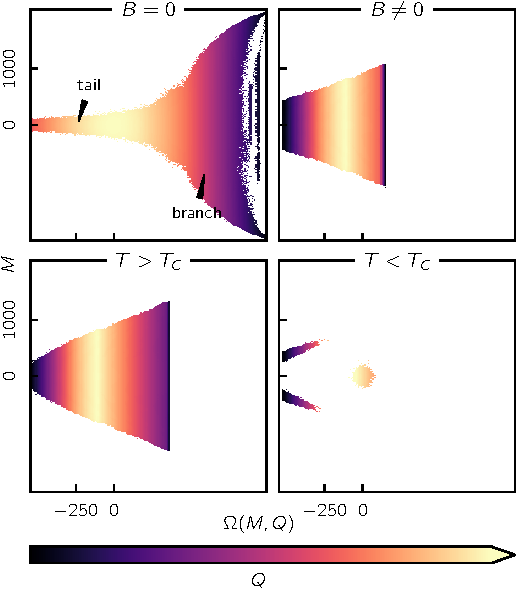
\includegraphics[width=1.05\linewidth]{figures/density_omega.pdf}
    \end{center}
    \caption{Here we computed the density of state estimation using \textbf{WHAM} for 4 different typical cases on a $L = 32$ size Ising model. To obtain this estimation we compiled all the datasets used for our previous studies including several starting configuration (\texttt{all-spin-up}, \texttt{all-spin-down}, \texttt{random}), different number of random walkers, and different random walk length. The Intermediate computation of the free energy used Thermodynamic Integration and Exponential averaging over all the data collected
    }
    \label{fig:density-states}
\end{figure}
However the exponential term in $\Omega_{\nu}(M,Q)$ can be a source of numerical instability, hence it is often replaced by the following relation : 
    \begin{equation*}
        \Omega_{\text{est}}(M,Q) \approx \frac{\sum_{\nu} N_{\nu}(M,Q)}
        {\sum_{\nu} N_{\nu} \e^{\beta(F_{\nu}- E_{\nu}(M,Q))}}
        \label{eq:WHAM2}
    \end{equation*}

In the figure \ref{fig:density-states} we can see the estimation of the density of states for the 2d ising model, it appears that the density of states for the zeros external field is close from the litterature one. Intersting things can be notice here, in the the case of $T<T_C$ the two branch of the magnetization valid in low magnetic external field vanish, this is probably due to the anti-ferromagnetic value of the coupling constant, decreasing other weights. One can verify that we recover the two branches (metastable state) when we compute the density only with positive value of the coupling constant. 

For $T>T_C$ one can see that external magnetic field will broaden the distribution in the "tail" of the density of states,which seems totally correct since magnetized state are more probable in non vanishing magnetic field, here we also lose the branches of the magnetization which is physically correct (we can verify that removing the anti-ferrmoagnetic contribution). 

This conlude our study on the 2d ising model and more globally on this introduction to computationnal statistical physics. Some concerns should be raise about free energy calculation since we absolutely need to do not have large unexplored domain of the phase space, to compute it. In order to do so one can design clever method to avoid being trapped in some region of the phase space wuile simulating (paralell tempering, cluster algorithm, multicanonical sampling \dots), but we will not discuss this here, and let the reader refer to the litterature for more information.


    \nocite{*}
    \printbibliography

\end{multicols}

\end{document}
